\documentclass[12pt, english]{article}

\usepackage[utf8]{inputenc}
\usepackage[T1]{fontenc}
\usepackage[english]{babel}

\selectlanguage{english}
% \usepackage{color}
% \usepackage[backend=biber]{biblatex}
% \usepackage{english}
% \usepackage{hyphenat}
\usepackage{graphicx}
% \usepackage{csquotes}
% \usepackage[makeroom]{cancel}
% \usepackage{amsmath}
% \addbibresource{bibliography.bib}

\DeclareUnicodeCharacter{00A0}{~}

\author{
	\begin{tabular}{r|l}
        Adam Jóźwiak& 216786@edu.p.lodz.pl\\
        Jan Klamka& 216797@edu.p.lodz.pl\\
        Piotr Pilecki& 216865@edu.p.lodz.pl\\
        Maciej Pracucik& 216869@edu.p.lodz.pl\\
        Tomasz Witczak& 216920@edu.p.lodz.pl\\
    \end{tabular}
}

\title{\huge \textbf{Ohunkakan}\\
\vspace{12pt}
\large \emph{Technical Design Document}\\
\large \emph{Game Engine Programming, 2020}
}

\begin{document}
\maketitle

\tableofcontents

\section{Requirements and features}

\begin{itemize}
	\item procedurally generated endless scene
	\item conversion and loading Unity scenes
	\item fire effect simulation
	\item various post-processing effects
	\item AABB collision detection and resolution
	\item multiple point lights
	\item scene graph with dirty flag
	\item simple GUI (buttons and text)
	\item external scene editor
	\item game logic encapsulated in .dll scripts
	\item skinned animations
	\item PBR renderer
	\item 3D sound
	\item basic game state machine
\end{itemize}

\section{Engine architecture}

\begin{figure}
	\centering
	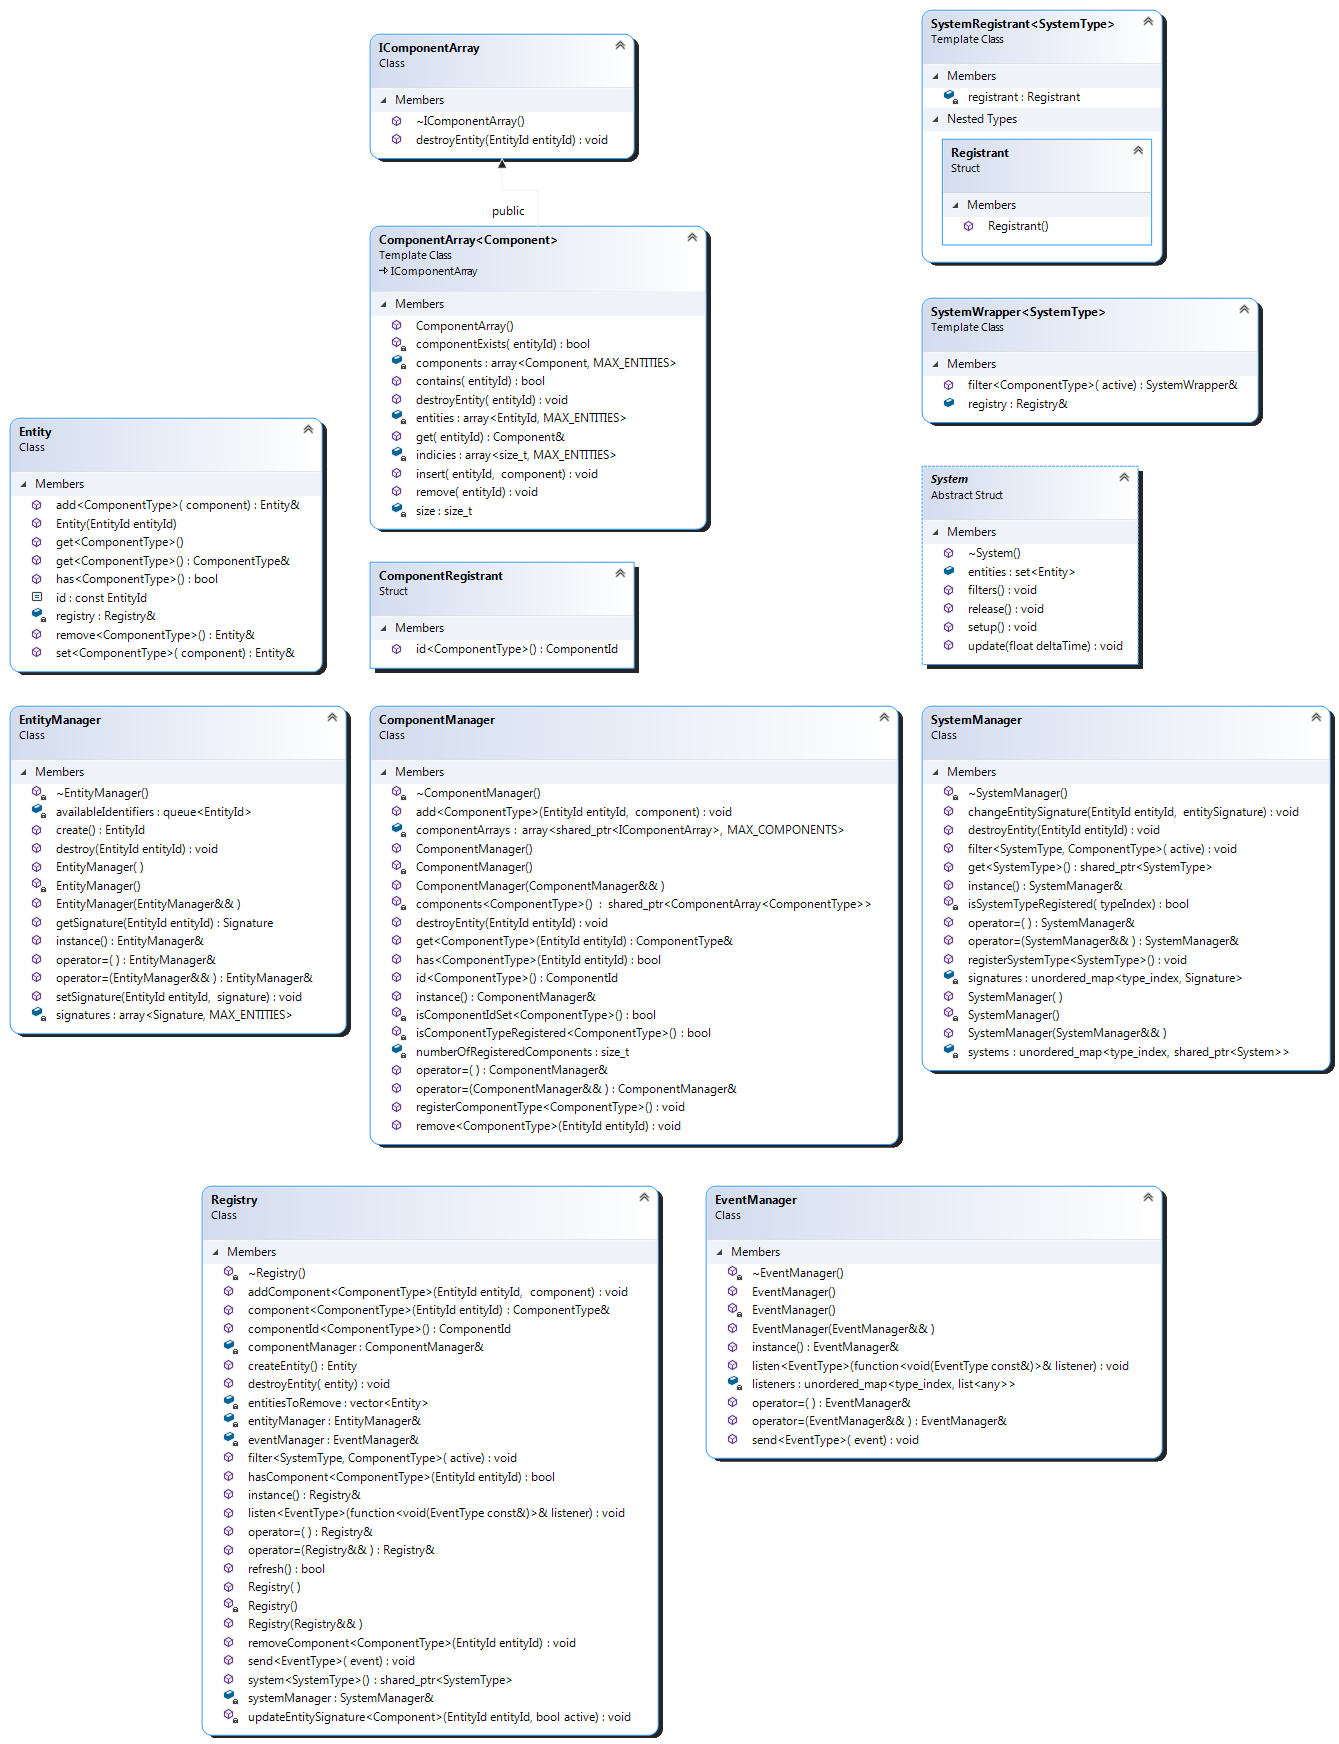
\includegraphics[width=\textwidth, height=0.9\textheight, keepaspectratio]{ecs.png}
	\caption{ECS architecture and event system}
	\label{figure_ecs_event}
\end{figure}


\subsection{ECS}

\subsubsection{Overview}
The ECS system used in our engine is purely based on components. The entities
are only identifiers and components are stored in the appropriate arrays in
component manager.

This system is the core of the engine. It allows us to decouple various
operations that could be done by putting them in separate systems. The
components that we used are loosely based on the ones found in the Unity
engine.

The event system is integrated with ECS for the simplicity of usage.

All managers implement a singleton pattern for a simpler API usage and
mitigating the access issues.

\subsubsection{Entity}
The entity itself is just a number, unsigned integer to be precise.

There is a maximum number of entities that can be created and it is defined by
the appropriate macro.

The EntityManager class handles the entity-related operations. It's responsible
for creating and destroying entities, as well as accessing the component
signature which stores the information about the components that the chosen
entity has.

Entities, as stated before, are only integers. Because of that, there is a
queue containing all the available identifiers, filled at startup. Then,
whenever the user wants to create an entity, the element (identifier) is popped
from the queue and returned to the user. Whenever the programmer wants to
destroy the entity, the operation is performed in reverse - the identifier gets
put back onto the queue.

The signature that stores the information about the component that an entity
has is a bitset. When an entity has the specific component, the corresponding
bit is set to one. When it doesn't, it's set to zero.


\subsubsection{Component}

There is no inheritance hierarchy if it comes to components. Each component
should be a POD struct. The information that a struct is a component is done
with metaprogramming and templates.

Each component has its own identifier which needs to be manually set by the
programmer when creating a component class. The identifier is stored as a
template specialisation of the member function of the ComponentRegistrant
class. In that way, we can have a different return value for the method that
depends solely on the type of the component.

After setting the identifier, each component must be registered manually by
invoking the registration function of the component manager which creates the
array for the components of the chosen type.

There is a custom class that represents the array of components. It's
implemented to an interface so that it can be stored and accessed by the
manager. The components are stored in a plain simple array of the chosen type.
This ensures that there is no dynamic allocation at runtime. All of the memory
is being statically allocated which means that that system will be faster than
the dynamic one.

The main point of storing the components in a static array is to have it be
tightly packed. To achieve that whenever the component is removed from the
array, the last element in the array is copied in the place of the deleted one.

The array that stores the components works a bit like a map but with the entity
identifier as a key.

\subsubsection{System}

Each system needs to inherit from the base system class. The base class
contains a set of all the entities that fit into the filtering criteria. It
also exposes the interface for the system that allows the user to do the setup,
cleanup, set the filters and do the update.

Systems work based on filters. A filter is just another component signature but
this time it's not used to specify which component an entity has. This time it
tells us which entities we want to have in our system container. It filters
only these entities that have the specified set of components. It does it by
comparing the signatures of the systems and components and then updating the
entity sets in systems.

Systems also need to be registered but this time the process is automatic. Each
system inherits from the SystemRegistrant template class which has a one static
object of the Registrant class. In the constructor of said object, we call the
registering function of the system manager. The fact that this object is static
tells us that the registration process will happen only once per type.

The registration creates the instance of the appropriate system in the system
manager. The systems are stored in a map that takes the type identifier as a
key and stores the value of a pointer to the system base class.

\subsubsection{Registry}
To keep it simple, Registry serves as a facade to all the managers. It wraps
all the important operations and provides the user with a simple interface.

With the registry, the users can create and destroy entities, manage addition
and deletion of components, set the system filters and also set up the event
system. Registry also serves an important function of synchronizing all the
managers with the up-to-date signatures of systems and entities.

\subsubsection{Utility}
For even simpler usage, there exists the Entity class that acts as a thin
wrapper around the entity identifier. It enables the user to write in a simpler
syntax by omitting the registry and using the methods of the entity itself. As
a result, all the operations that one would want to perform on the entity or
its components can be done with the entity object only. The usage of singletons
for managers allows for this type of free access, regardless of the place in
the program where it's being called.

\subsection{Events system}
Each event, just like component, can be just a POD type.

First thing that needs to be done when the user wants use the event system is
to register the listeners. They can be just free functions or even members of
classes. Then with the access to the Registry class, the user can just send the
event object through the appropriate send method. The manager then iterates
over its listener container and calls the functions that listen to that
specific type of an event.

\section{Entities}
\begin{itemize}
	\item Terrain
	      \begin{itemize}
		      \item Grass
		      \item Tree
		      \item Ground
		      \item Rocks (walls, obstacles, decorations)
	      \end{itemize}
	\item Billboards
	      \begin{itemize}
		      \item Flame
		      \item Enemies
		            \begin{itemize}
			            \item Bishop
			            \item Rook
			            \item Enemy moving sideways
			            \item Enemy moving back and forward
			            \item Enemy moving up and down
		            \end{itemize}
	      \end{itemize}
	\item Enemy AI boundaries
	\item Level colliders
	\item Traps
	\item Waterfalls
	\item UI elements
	      \begin{itemize}
		      \item Buttons
		      \item Text
	      \end{itemize}
	\item Player
\end{itemize}


\section{Components}

\begin{figure}
	\centering
	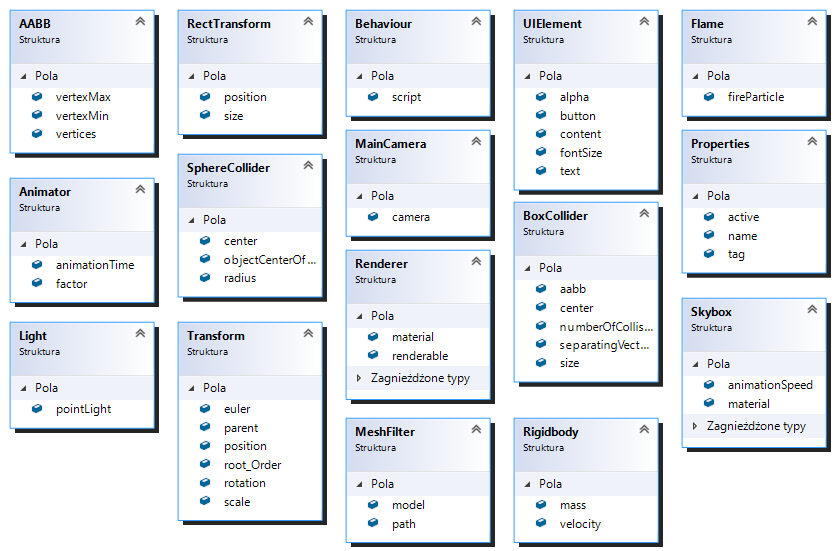
\includegraphics[width=\textwidth]{image7.png}
	\caption{Components}
	\label{figure_components}
\end{figure}


\subsection{AABB}
It defines two points in the space corresponding to model’s minimum and maximum
vertex position values on every axis. It's used for creating the box colliders.

\subsection{Animator}
It contains the information about the duration and the velocity of the
animation.

\subsection{Behaviour}
It adds the behaviour scripts to entities for defining the object logic.

\subsection{BoxCollider}
It adds the bounding box for collision detection. Whenever the collider surface
intercepts with a different one, collider system sends an event that later can
be resolved in a specific behaviour script.

\subsection{Flame}
It adds an animated fire particle billboard.

\subsection{Light}
It attaches a point light to the entity.

\subsection{MainCamera}
It defines the main camera used in the game.

\subsection{MeshFilter}
It adds a model to the entity and contains the information about the file path
in the project files.

\subsection{Properties}
It contains the information about the name and the tag of the entity. It also
defines whether it is active in the scene.

\subsection{RectTransform}
It defines the position in the scene and the size of the UI element.

\subsection{Renderer}
It contains the information about the material properties, such as paths to the
appropriate textures and heights used in parallax mapping.

\subsection{Rigidbody}
It defines the mass and the velocity of the entity and decides whether it is
going to be affected by the physics system.

\subsection{Skybox}
It contains the information about the textures that create a cube map and the
animation speed defining how quickly the skybox will be animated.

\subsection{SphereCollider}
It adds a bounding sphere that's used for detecting the collision by checking
whether the distance between the colliding object and the center of the sphere
collider is smaller than the value of the sphere radius.

\subsection{Transform}
It contains the information about the position of the object, the rotation and
the scale in the world.

\subsection{UIElement}
It defines whether or not the entity is a UI element and what type of an
element it is, e.g. text or button.

\section{Systems}

\begin{figure}
	\centering
	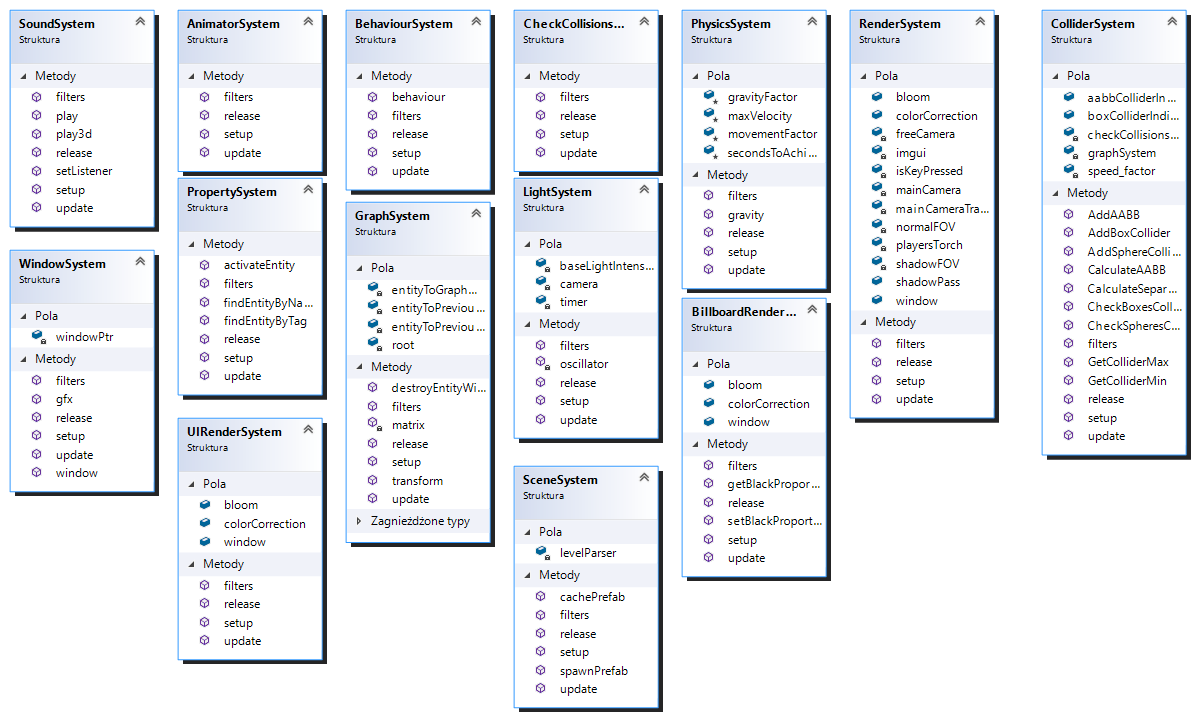
\includegraphics[width=\textwidth]{image6.png}
	\caption{Systems}
	\label{figure_systems}
\end{figure}

\subsection{Animator}

This system is responsible for advancing the animation times for these models
which should be animated.

\subsection{Behaviour}

It's a system for handling behaviour scripts, e.g. CameraController. It runs
their updates but also loads the appropriate \textit{.dll}’s at the game
startup.

\subsection{BillboardRender}

This system is responsible for rendering billboards, i.e. flames and enemies.
It also sets and updates their positions in the world. The system contains the
last post-processing passes and because of that it exposes the interface to set
the black fade effect in the color correction post-process.

\subsection{CheckCollision}

The sole purpose of this system is to act as a filter for the entities that
should be taken into account when checking collisions. The filtered objects are
then used in the ColliderSystem.

\subsection{Collider}

It's a system which exposes specific methods for handling all things related to
collisions. It enables creating and updating the colliders (boxes and spheres)
as well as checking and resolving collisions. It is also used for frustum
culling with its AABB functionality.

\subsection{Graph}

This system implements the scene graph with the dirty flag. It maintains a
graph structure of all the entities and checks whether or not its transform or
activity status have changed since the last frame. In that case, the transform
matrices are recalculated. The system also exposes the interface for all the
other systems to access the cascaded model transformation matrix that includes
the hierarchy between objects. Whats more, it also has a method for deleting
entities with respect to that hierarchy.

\subsection{Light}

It handles updates related to lights in the scene. It is used for setting and
updating their positions as well as adding an oscillatory flicker effect to
their intensity level.

\subsection{Physics}

The purpose of this system is to handle the gravity for the objects that need it.

\subsection{Property}

Although it's a system, it doesn't function as one. The only purpose of it is
to expose the interface for looking for entities by their name or tag.
Furthermore, it has a method for enabling or disabling the entity but, on the
contrary to the graph system, it bypasses the hierarchy of objects and affects
the entity only.

\subsection{Render}

It is responsible for rendering all entities in the scene. It performs frustum
culling so only the entities that are inside the viewing frustum are rendered.
It also renders point shadows and starts applying the post-processing effects
such as bloom. The next part of the rendering pipeline is then continued in the
billboard rendering system.

\subsection{Scene}

It's a system for loading the startup scene. It is also responsible for
spawning prefabs or caching them which is useful when applied to world chunks.

\subsection{Sound}

This system handles the sound effects. It loads and caches their files at
startup. Every frame it updates the 3D sound source positions. Moreover, the
system exposes a few basic methods for playing sounds that could be used for
example in the scripts.

\subsection{UIRender}

It's the last system in the rendering pipeline of the engine. Following after
the billboard system, its responsibility lies in rendering every UI element in
the scene, e.g. buttons or text. It also ends the frame render which performs
the buffer swap.

\subsection{Window}

This system creates the game window, sets its resolution and the name but also
makes the window pointer available for the other systems to use.

\section{Events}

\begin{figure}
	\centering
	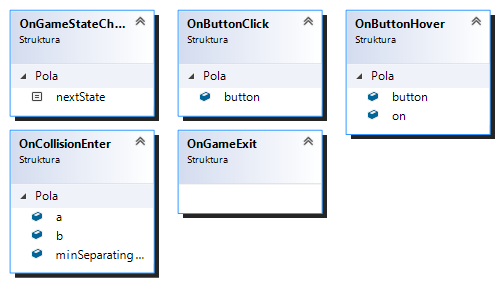
\includegraphics[width=\textwidth]{image2.png}
	\caption{Events}
	\label{figure_events}
\end{figure}

\subsection{OnButtonClick}
After a button is clicked on with the mouse, this event is being sent with the
information about the button.

\subsection{OnButtonHover}
It is sent whenever the player hovers over a button using the mouse.

\subsection{OnCollisionEnter}
In case collider system detects a collision, it sends this event so that later
it can be reacted to by the programmer e.g. in the behaviour scripts.

\subsection{OnGameExit}
After the player decides to exit the game, this event is being sent to the main
engine script responsible for the main gameplay logic. What follows after is
the release of all the systems and then the game exits.

\subsection{OnGameStateChange}
Whenever one of the predefined game states has changed (for example when player
clicks the ''Play'' button in the menu to transition into the game), this event
is responsible for informing multiple systems in which state the game is
currently in.

\section{Scripts}

\subsection{CameraController}
It's responsible for controlling the camera behaviour, switching its position
depending on the game state, following the player while playing, shaking the
camera to imitate the effect of the cave collapsing.

\begin{figure}
	\centering
	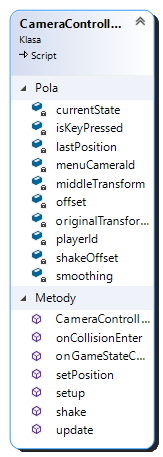
\includegraphics[width=\textwidth, height=0.9\textheight, keepaspectratio]{image3.png}
	\caption{CameraController script}
	\label{figure_cameracontrollerscript}
\end{figure}

\subsection{EnemyController}
It's responsible for controlling the enemies, their movement and the way of
interacting with the environment.

\begin{figure}
	\centering
	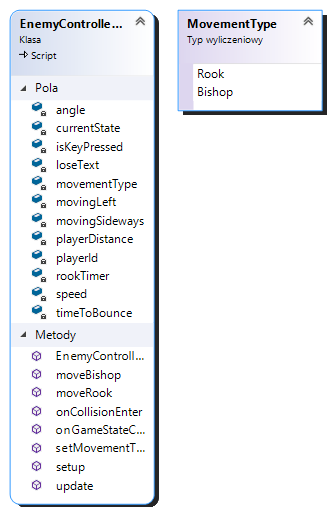
\includegraphics[width=\textwidth, height=0.9\textheight, keepaspectratio]{image5.png}
	\caption{EnemyController script}
	\label{figure_enemycontrollerscript}
\end{figure}

\subsection{GameManager}
It's responsible for the main gameplay logic, i.e. generating the level
procedurally, spawning the enemies, the torches, maintaining the proper UI
state, switching the game states when needed, etc.

\begin{figure}
	\centering
	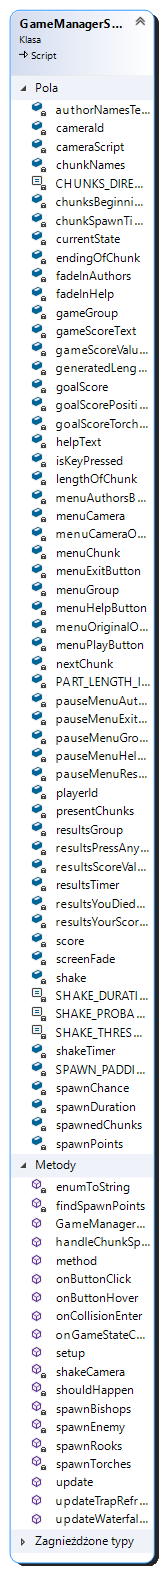
\includegraphics[width=\textwidth, height=0.9\textheight, keepaspectratio]{image1.png}
	\caption{GameManager script}
	\label{figure_gamemanagerscript}
\end{figure}

\subsection{PlayerController}
It's responsible for controlling the player, his movement, switching of the
forms, interacting with traps, waterfalls, enemies and torches. It also defines
the light emitted by the player and its behaviour.

\begin{figure}
	\centering
	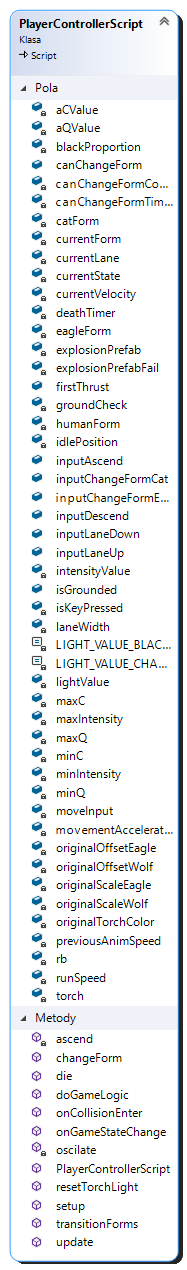
\includegraphics[width=\textwidth, height=0.9\textheight, keepaspectratio]{image4.png}
	\caption{PlayerController script}
	\label{figure_playercontrollerscript}
\end{figure}

\section{Tools}

\subsection{Unity}
\begin{itemize}
	\item Setting up the main scene
	\item Creating the UI
	\item Creating the layout of game levels as predefined chunks
	\item Preparing the assets, e.g. textures, models, materials, fonts, etc.
	\item Storing chunk properties for the in-game procedural generation
	      mechanism
	\item Creating the prefabs for further processing
	\item Tagging the objects
\end{itemize}

\subsection{Utility conversion script}
\begin{itemize}
	\item Converting Unity files (such as: .scene, .prefab, .mat, .meta) to our format
	\item Performing batch conversions
	\item Copying the asset files around the repository
\end{itemize}

\subsection{Assimp}
\begin{itemize}
	\item Loading 3D models (mainly .fbx, .dae, .gltf formats)
	\item Loading the necessary information for skinning, e.g. bone identifiers and
	      weights, animation names and durations
\end{itemize}

\subsection{SoLoud}
\begin{itemize}
	\item Loading the sounds (mainly in .wav format)
\end{itemize}

\subsection{ImGUI}
\begin{itemize}
	\item Assisting in the debugging process
\end{itemize}

\subsection{3ds Max / Blender}
\begin{itemize}
	\item Modeling the characters
	\item Texturing the meshes
	\item Setting up the bones for the models
	\item Skinning
	\item Animating
	\item Converting between formats
\end{itemize}

\subsection{Photoshop}
\begin{itemize}
	\item Creating and processing textures for PBR materials and other uses
\end{itemize}

\section{Rendering techniques}
\subsection{Physically Based Rendering}
PBR is a technique for real-time realistic lighting. It's based on the information contained in these sets of textures: albedo, ambient occlusion, metalness and roughness. They all keep information that is then used to calculate the radiance of the light. We use the Cook-Torrace BRDF function, the Fresnel-Schilck operation and Smith's geometry method. What makes this physically based is the fact, that the calculations are based on the BRDF function, they use the model of microfacets and they obey the laws of energy conservation. Overall, the results are far better than the ones achieved with the simpler Lambert-Phong models.

\subsection{Normal mapping}
It's a technique for extending the usage of normal vectors for even better results with the lighting.

The normal and tangent vectors are passed for every vertex of the model. Then in the pixel shader we construct the TBN matrix which is used to create a transformation from tangent to the world space. The normal vector is then read from the normal map texture, properly converted to the [-1,1] range of values and then transformed to the world space to be used with lighting algorithms.

The TBN matrix is constructed by putting the normal, tangent and bitangent vectors as columns of the matrix. The vectors then serve as the base of the new affine subspace.

What's interesting is that if these vectors are normalized then the resulting TBN matrix is orthogonal which can be used when wanting to find the inverse of the matrix. We can then just calculate it by doing the transposition.

There's a big leap in terms of quality of the rendered models when using normal mapping, yet it's just a slight illusion which breaks when looking at object from an angle. We then see that the geometry is not changed but nonetheless the effect provides us with great results.

\subsection{Parallax mapping}
The variant of the algorithm that we used here is called Parallax Occlusion Mapping.

Firstly, we calculate the maximal offset of the step we are going to be taking with our texture coordinates. Then we can calculate the number of samples taken depending on the angle of viewing - the larger the angle the more samples we're going to be using.

The whole premise of the algorithm is simple. We take the height/depth map and after transforming the view vector into the tangent space we can perform a stepwise sampling along the direction of the view. We do it in a loop. Take a step. Each step taken is translated into a step in the UV space. Then sample the depth map at that point. Check if we already "crossed" the surface. If not, keep going deeper. Otherwise, interpolate the last two steps and return the new texture coordinate for the parallax-mapped surface.

The effect is best used on plain surfaces. We used it on the ground tiles for the extra level of depth (contrary to normal mapping, parallax simulates the displacement of the geometry).

\subsection{Billboarding}
To render a billboard, the position of one vertex in the world has to be
defined.  Then its position is being passed on to the geometry shader, that
reads texture dimensions and then creates three additional vertices from which
the billboard will be created; also taking into the account the position of the
main camera, so that the image always faces it.

\subsection{Fire effect}
It is a billboard containing one of the following: albedo texture, noise
texture, gradient texture and a mask texture. For a more randomized output look
of the flame, the noise texture is used three times with different x and y
offsets.  Both albedo and mask textures are being transformed over time to
create the effect of a ''wobbling'' fire. Depending on how much of a specific
red, green or blue color is needed to be highlighted, three different values
may be adjusted to get a different looking flame. In the end the flame is
clipped to the shape defined by the mask texture.

\subsection{Enemy effect}
The effect of the enemy is created in a very similar manner to the fire effect,
with slight differences in pixel shader code regarding the offsets to a
different set of textures and values multiplying the ''animation'' speed.
Unlike the fire effect, here the mask is not being transformed which gives us a
sturdy image with animated insides.

\subsection{Skinning}
The model for animations is loaded via Assimp library -- all the meshes and
nodes loaded by it are converted into classes. Assimp also loads the necessary
information for animating the model, such as bones identifiers and weights.
When the animation is selected, bones are being interpolated between each
keyframe, creating the desired animation effect.

\subsection{Bloom}
The renderer creates two render targets for the scene. One of them needs to be
saturated because we want to extract the bright objects. Then we use Gaussian
blur on that texture. The next step is adjusting the saturation using the
linear interpolation. After this the texture with bloom is combined with the
original color.

\subsection{Color correction}
The used algorithms for color correction are brightness and contrast adjustments, gamma correction and curves based on the input LUT texture.

\subsection{Frustum culling}
To create the frustum we need six planes. Before each frame every entity in
scene graph needs to be checked if it should be rendered. To be shown on the
screen, the entity has to be inside the frustum or collide with it (for
collision detection we use the AABB bounding boxes).

\subsection{Shadow mapping (point lights)}
The cube map is first created as a set of six render targets. In the shadow pass, we render the scene to each of the directions of the cube map. In that rendering pass, we calculate the depth of the fragment. Then, in the lighting pass, we can use the information stored in the depth cube map to compare the actual depth of the rendered fragment and decide whether or not the fragment should be lit or covered in shadow.

% \printbibliography

\end{document}
